% Supplementary material for the compact v12 manuscript.

\documentclass[10pt]{article}
\usepackage[T1]{fontenc}
\usepackage[letterpaper,margin=0.78in]{geometry}
\usepackage{graphicx}
\graphicspath{{./}{../}}
\usepackage{booktabs}
\usepackage{tabularx}
\usepackage{array}
\usepackage{ragged2e}
\newcolumntype{Y}{>{\RaggedRight\arraybackslash}X}
\usepackage{caption}
\usepackage{float}
\usepackage{amsmath}
\usepackage{hyperref}
\captionsetup{font=footnotesize,labelfont=bf}
\renewcommand{\thefigure}{S\arabic{figure}}
\renewcommand{\thetable}{S\arabic{table}}
\setlength{\parindent}{1em}
\setlength{\parskip}{0.25em}
\setlength{\textfloatsep}{8pt plus 2pt minus 2pt}
\setlength{\floatsep}{8pt plus 2pt minus 2pt}
\sloppy

\begin{document}

\begin{center}
{\Large\bfseries Supplementary Material}\\[0.3em]
{\large Recurrent Connection Topology Supports Reactive Control through Propagation Dynamics in Fixed-Weight Spiking Neural Networks}
\end{center}

\section*{S1. Statistical Boundary for TO/TG/TI Controls}

The main text uses the CartPole TO/TG/TI control as a final best-fitness audit
under an aligned evolutionary protocol, and the MountainCar TO/TG/TI control as
a strict 20-episode final-evaluation audit. To make this endpoint boundary
explicit, the release artifact contains seed-level tables with both CartPole
best-fitness and strict 20-episode re-evaluation fields, plus the script used to
compute the confidence intervals below.

We also ran a two-one-sided-tests (TOST) sensitivity audit to avoid interpreting
non-significant NHST results as unrestricted equivalence. Margins are
illustrative and stated explicitly. On CartPole, TO--TI is not supported under a very tight
$\delta=2$ step margin but is supported under $\delta=5$ steps. On
MountainCar, TO--TI is not supported under $\delta=300$ shaped-fitness units
and is supported only under the broad $\delta=500$ margin.

\IfFileExists{artifact/processed_results/supplement_table_to_tg_ti.tex}{%
  \begin{table}[H]
\centering
\footnotesize
\caption{\textbf{Statistical boundary for TO/TG/TI controls.} Mean confidence intervals and pairwise Welch mean-difference intervals are computed from seed-level final scores. They define the range of differences compatible with the data and are not formal equivalence or non-inferiority tests.}
\label{tab:supp-stat-boundary}
\begin{tabularx}{\textwidth}{@{}llYYY@{}}
\toprule
\textbf{Task} & \textbf{Condition / contrast} & \textbf{Mean or diff. (95\% CI)} & \textbf{Median [IQR]} & \textbf{Success / goal rate} \\
\midrule
CartPole & TO & $498.1$ [$496.0$, $500.2$] & $500.0$ [$497.1$, $500.0$] & 10/10 \\
CartPole & TG & $496.8$ [$494.2$, $499.3$] & $497.6$ [$493.5$, $500.0$] & 10/10 \\
CartPole & TI & $497.8$ [$495.3$, $500.3$] & $500.0$ [$495.5$, $500.0$] & 10/10 \\
CartPole & TO-TI & $0.2$ [$-2.8$, $3.3$] & -- & -- \\
CartPole & TO-TG & $1.3$ [$-1.8$, $4.4$] & -- & -- \\
CartPole & TG-TI & $-1.1$ [$-4.4$, $2.2$] & -- & -- \\
\midrule
MountainCar & TO & $895.5$ [$648.8$, $1142.2$] & $763.4$ [$658.6$, $798.4$] & 16/20; goal 17.0\% \\
MountainCar & TG & $1049.4$ [$774.0$, $1324.8$] & $764.0$ [$682.4$, $1243.0$] & 17/20; goal 17.8\% \\
MountainCar & TI & $984.0$ [$703.7$, $1264.3$] & $764.0$ [$679.0$, $992.9$] & 16/20; goal 15.5\% \\
MountainCar & TO-TI & $-88.5$ [$-449.9$, $272.8$] & -- & -- \\
MountainCar & TO-TG & $-153.9$ [$-511.6$, $203.8$] & -- & -- \\
MountainCar & TG-TI & $65.4$ [$-314.7$, $445.4$] & -- & -- \\
\bottomrule
\end{tabularx}
\end{table}
%
}{%
  \begin{table}[H]
\centering
\footnotesize
\caption{\textbf{Statistical boundary for TO/TG/TI controls.} Mean confidence intervals and pairwise Welch mean-difference intervals are computed from seed-level final scores. They define the range of differences compatible with the data and are not formal equivalence or non-inferiority tests.}
\label{tab:supp-stat-boundary}
\begin{tabularx}{\textwidth}{@{}llYYY@{}}
\toprule
\textbf{Task} & \textbf{Condition / contrast} & \textbf{Mean or diff. (95\% CI)} & \textbf{Median [IQR]} & \textbf{Success / goal rate} \\
\midrule
CartPole & TO & $498.1$ [$496.0$, $500.2$] & $500.0$ [$497.1$, $500.0$] & 10/10 \\
CartPole & TG & $496.8$ [$494.2$, $499.3$] & $497.6$ [$493.5$, $500.0$] & 10/10 \\
CartPole & TI & $497.8$ [$495.3$, $500.3$] & $500.0$ [$495.5$, $500.0$] & 10/10 \\
CartPole & TO-TI & $0.2$ [$-2.8$, $3.3$] & -- & -- \\
CartPole & TO-TG & $1.3$ [$-1.8$, $4.4$] & -- & -- \\
CartPole & TG-TI & $-1.1$ [$-4.4$, $2.2$] & -- & -- \\
\midrule
MountainCar & TO & $895.5$ [$648.8$, $1142.2$] & $763.4$ [$658.6$, $798.4$] & 16/20; goal 17.0\% \\
MountainCar & TG & $1049.4$ [$774.0$, $1324.8$] & $764.0$ [$682.4$, $1243.0$] & 17/20; goal 17.8\% \\
MountainCar & TI & $984.0$ [$703.7$, $1264.3$] & $764.0$ [$679.0$, $992.9$] & 16/20; goal 15.5\% \\
MountainCar & TO-TI & $-88.5$ [$-449.9$, $272.8$] & -- & -- \\
MountainCar & TO-TG & $-153.9$ [$-511.6$, $203.8$] & -- & -- \\
MountainCar & TG-TI & $65.4$ [$-314.7$, $445.4$] & -- & -- \\
\bottomrule
\end{tabularx}
\end{table}
%
}

\begin{table}[H]
\centering
\footnotesize
\caption{\textbf{TOST sensitivity audit for selected TO contrasts.} The table
reports two one-sided equivalence tests under explicitly stated margins. These
values are used as margin-sensitivity diagnostics, not as unrestricted
equivalence claims.}
\begin{tabular}{@{}llccc@{}}
\toprule
\textbf{Task} & \textbf{Contrast} & \textbf{Margin} & \textbf{$p_\mathrm{TOST}$} & \textbf{Minimum supported margin} \\
\midrule
CartPole & TO--TI & $\delta=2$ steps & $0.121$ & $2.76$ steps \\
CartPole & TO--TI & $\delta=5$ steps & $0.002$ & $2.76$ steps \\
CartPole & TO--TG & $\delta=5$ steps & $0.011$ & $3.87$ steps \\
MountainCar & TO--TI & $\delta=300$ & $0.122$ & $389$ \\
MountainCar & TO--TI & $\delta=500$ & $0.013$ & $389$ \\
MountainCar & TO--TG & $\delta=500$ & $0.029$ & $452$ \\
\bottomrule
\end{tabular}
\end{table}

\section*{S2. Additional Mechanistic Diagnostics}

\begin{figure}[H]
\centering
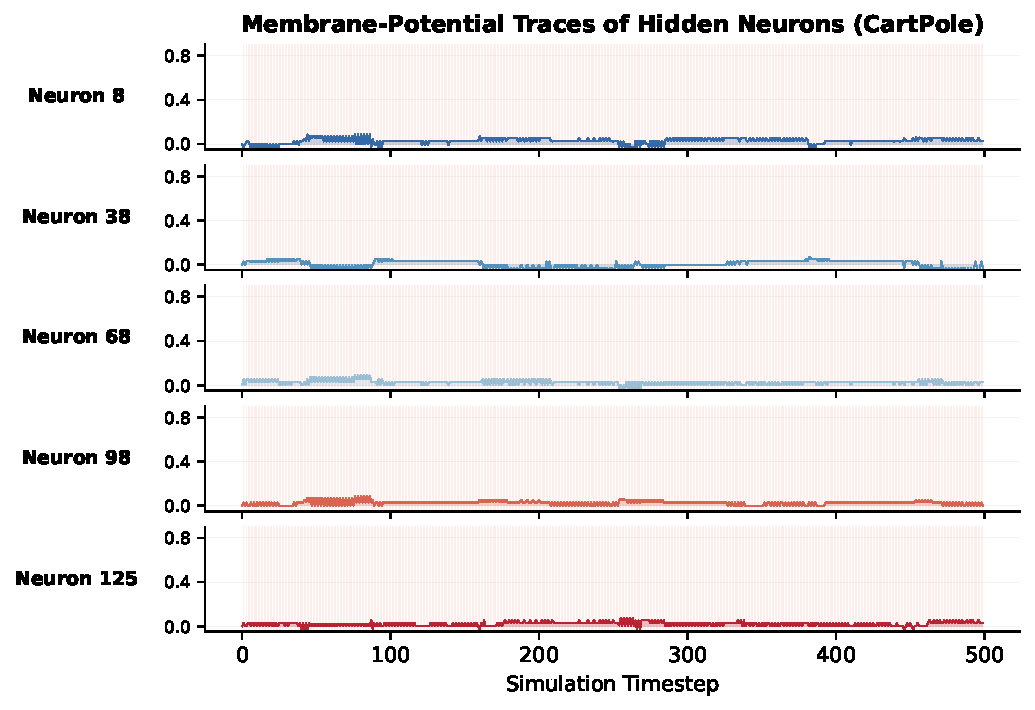
\includegraphics[width=0.92\linewidth]{figures_arxiv/fig03_membrane_traces.pdf}
\caption{\textbf{Membrane-potential trajectories (CartPole).} Membrane potential
of five representative hidden neurons (N8, N38, N68, N98, N125) over the first
500 simulation timesteps. The traces show sustained spiking activity rather
than relaxation to a stable equilibrium, consistent with the interpretation that
information is carried through ongoing temporal propagation rather than through
precise hidden membrane values alone.}
\end{figure}

\begin{figure}[H]
\centering
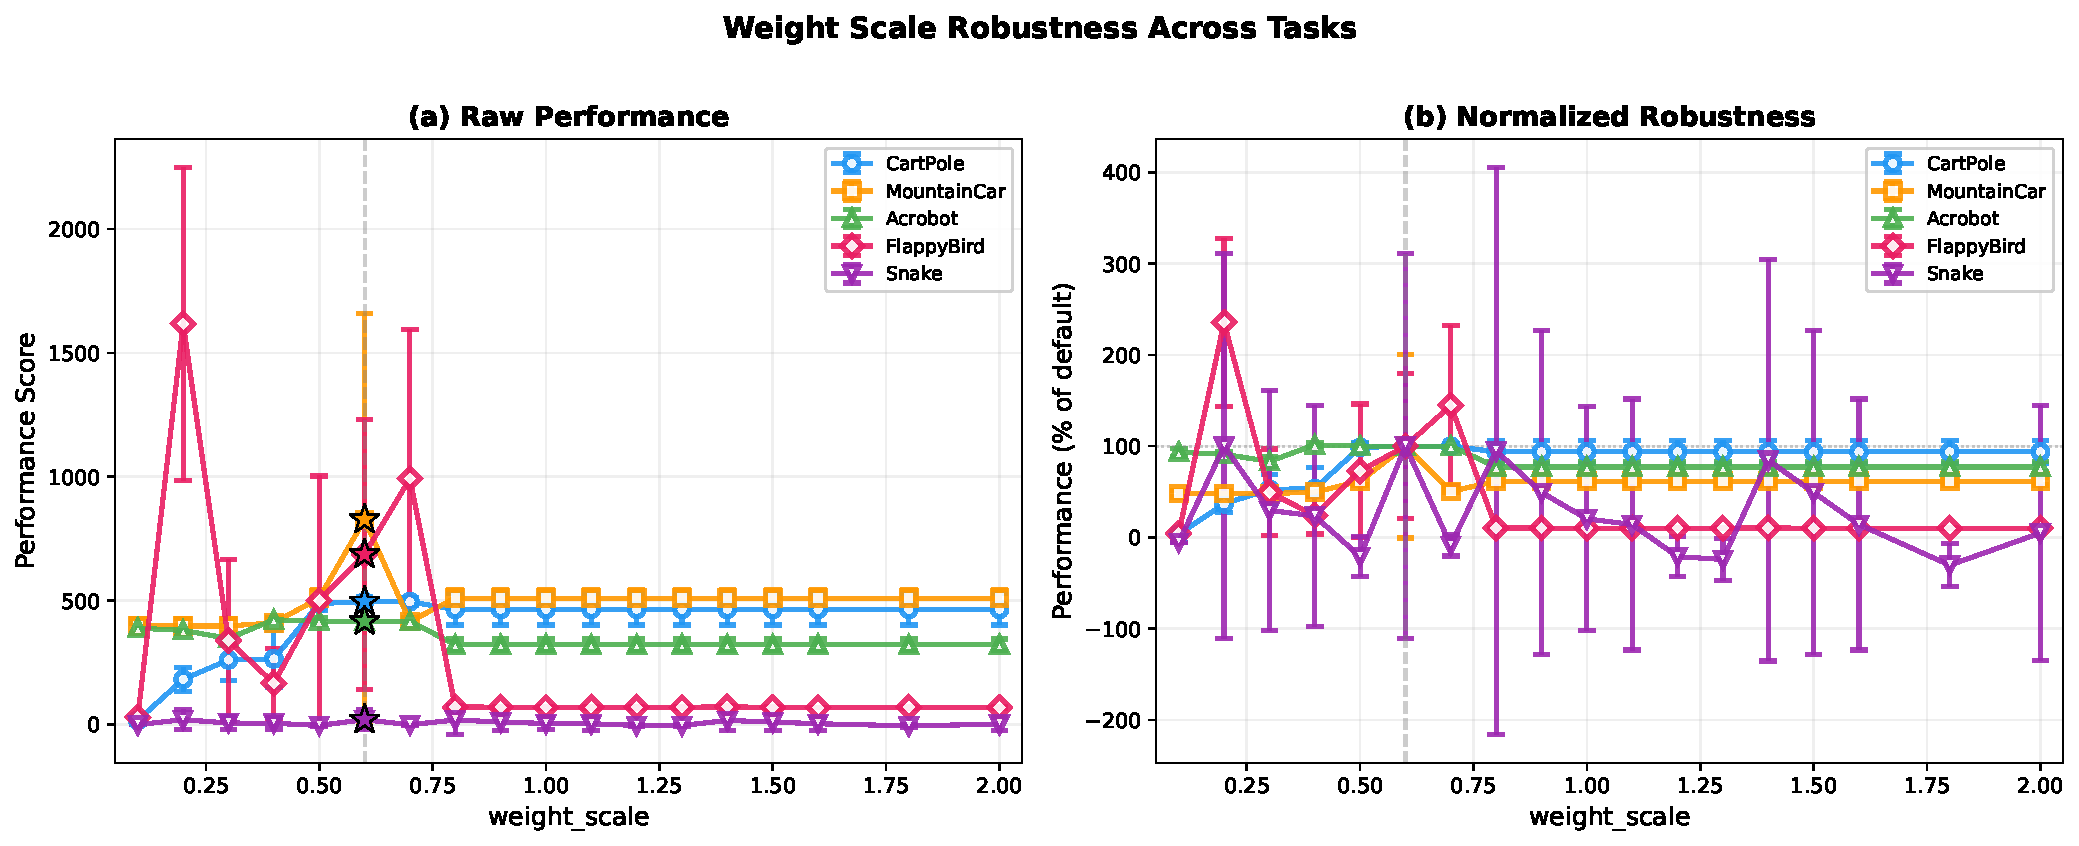
\includegraphics[width=0.92\linewidth]{figures_arxiv/fig05_weight_robustness.pdf}
\caption{\textbf{Post-hoc weight-scale sweep across discrete tasks.} The evolved
topology is evaluated while sweeping the single global weight scale after
training. The dashed line marks the default discrete-task scale ($0.6$). These
curves are diagnostic rather than a separate tuning protocol: the main
topology-only experiments hold the scale fixed during evolution and evaluation.}
\end{figure}

\begin{table}[H]
\centering
\footnotesize
\caption{\textbf{Non-spiking rate-substitution control.} The same evolved
CartPole topology, Dale signs, global scale, and $T_\text{steps}$ are evaluated
after replacing threshold-and-reset spiking with continuous rate nonlinearities
over a gain grid. This is a mechanistic substitution control, not a separately
evolved rate-network baseline.}
\begin{tabular}{@{}lcc@{}}
\toprule
\textbf{Controller} & \textbf{Best setting} & \textbf{20-episode score} \\
\midrule
Spiking LIF reference & threshold/reset & $460.2\pm61.6$ \\
Rate substitution & clipped ReLU, gain $0.5$ & $12.2\pm1.4$ \\
\bottomrule
\end{tabular}
\end{table}

\section*{S3. Structural Fingerprint Metadata Audit}

The five-task structural fingerprint analysis is configuration-separable, but
task identity is coupled to architecture metadata. A leave-one-out KNN classifier
using the 19 structural features reaches $94.0\%$ accuracy. However, the
architecture metadata $(N,n_\text{in},n_\text{out})$ alone classify task labels
at $100\%$ in this data set. After linearly residualizing the structural
features against these architecture metadata, LOO-KNN accuracy drops to
$48.0\%$. Within the fixed-$N=128$ subset (CartPole versus Acrobot), structural
features separate the two tasks at $100\%$, but this subset still differs in I/O
interface and contains only two tasks. These diagnostics support the main-text
restriction to configuration-identifiable, not architecture-independent,
fingerprints.

\section*{S4. Connection Ablation Diagnostics}

\begin{table}[H]
\centering
\footnotesize
\caption{\textbf{Systematic connection-type ablation results.} The CartPole
baseline is $415.4\pm18.6$ steps (mean of 20 episodes, 5 evaluations). Because
some ablations remove a large fraction of the graph and random-control variance
is high, specificity indices should be read descriptively.}
\begin{tabularx}{\textwidth}{@{}lYYYYY@{}}
\toprule
\textbf{Ablation condition} & \textbf{Edges deleted} & \textbf{Post-ablation perf.} & \textbf{Random-control perf.} & \textbf{Specificity index} & \textbf{Functional reading} \\
\midrule
\textbf{Delete E$\rightarrow$E} & 3,569 (53\%) & \textbf{9.3} & ${\sim}328$ & $+$0.12 & share too large; index descriptive \\
Delete I$\rightarrow$E & 1,303 (19\%) & 125.2 & ${\sim}314$ & $-$0.20 & arrangement not specific \\
Delete E$\rightarrow$I & 1,329 (20\%) & 137.9 & ${\sim}303$ & $-$0.21 & arrangement not specific \\
\textbf{Delete I$\rightarrow$I} & 484 (7\%) & \textbf{47.4} & ${\sim}259$ & undecidable ($+$0.27) & random-control variance too large \\
\bottomrule
\end{tabularx}
\end{table}

\begin{figure}[H]
\centering
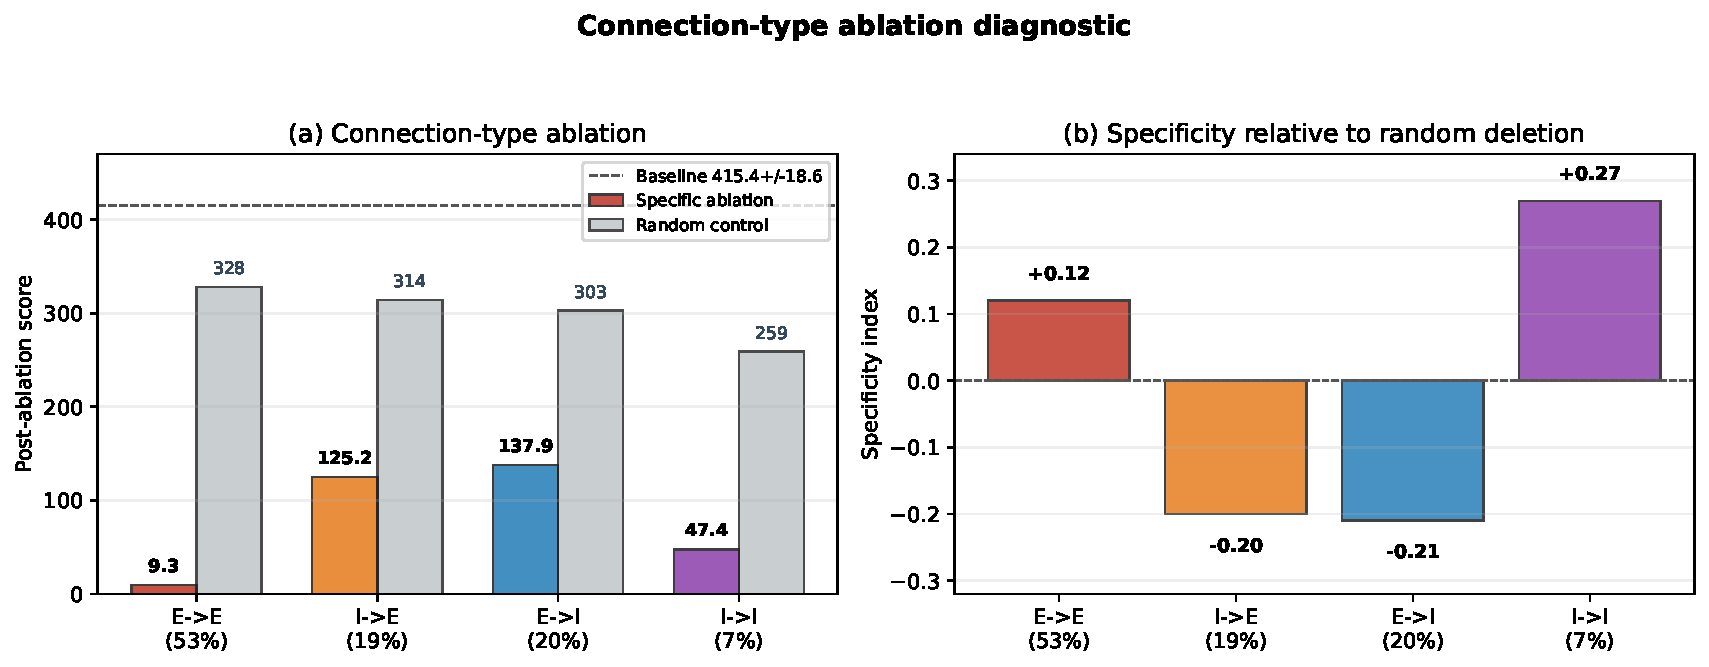
\includegraphics[width=0.92\linewidth]{figures_arxiv/fig07_connection_ablation.pdf}
\caption{\textbf{Connection-type ablation diagnostic.} Specific deletion of
E/I connection classes is compared with random deletion of the same number of
edges. The analysis supports the main-text conclusion that performance is not
explained by enrichment of a small local motif class.}
\end{figure}

\section*{S5. Transfer and Adaptation Diagnostics}

\begin{figure}[H]
\centering
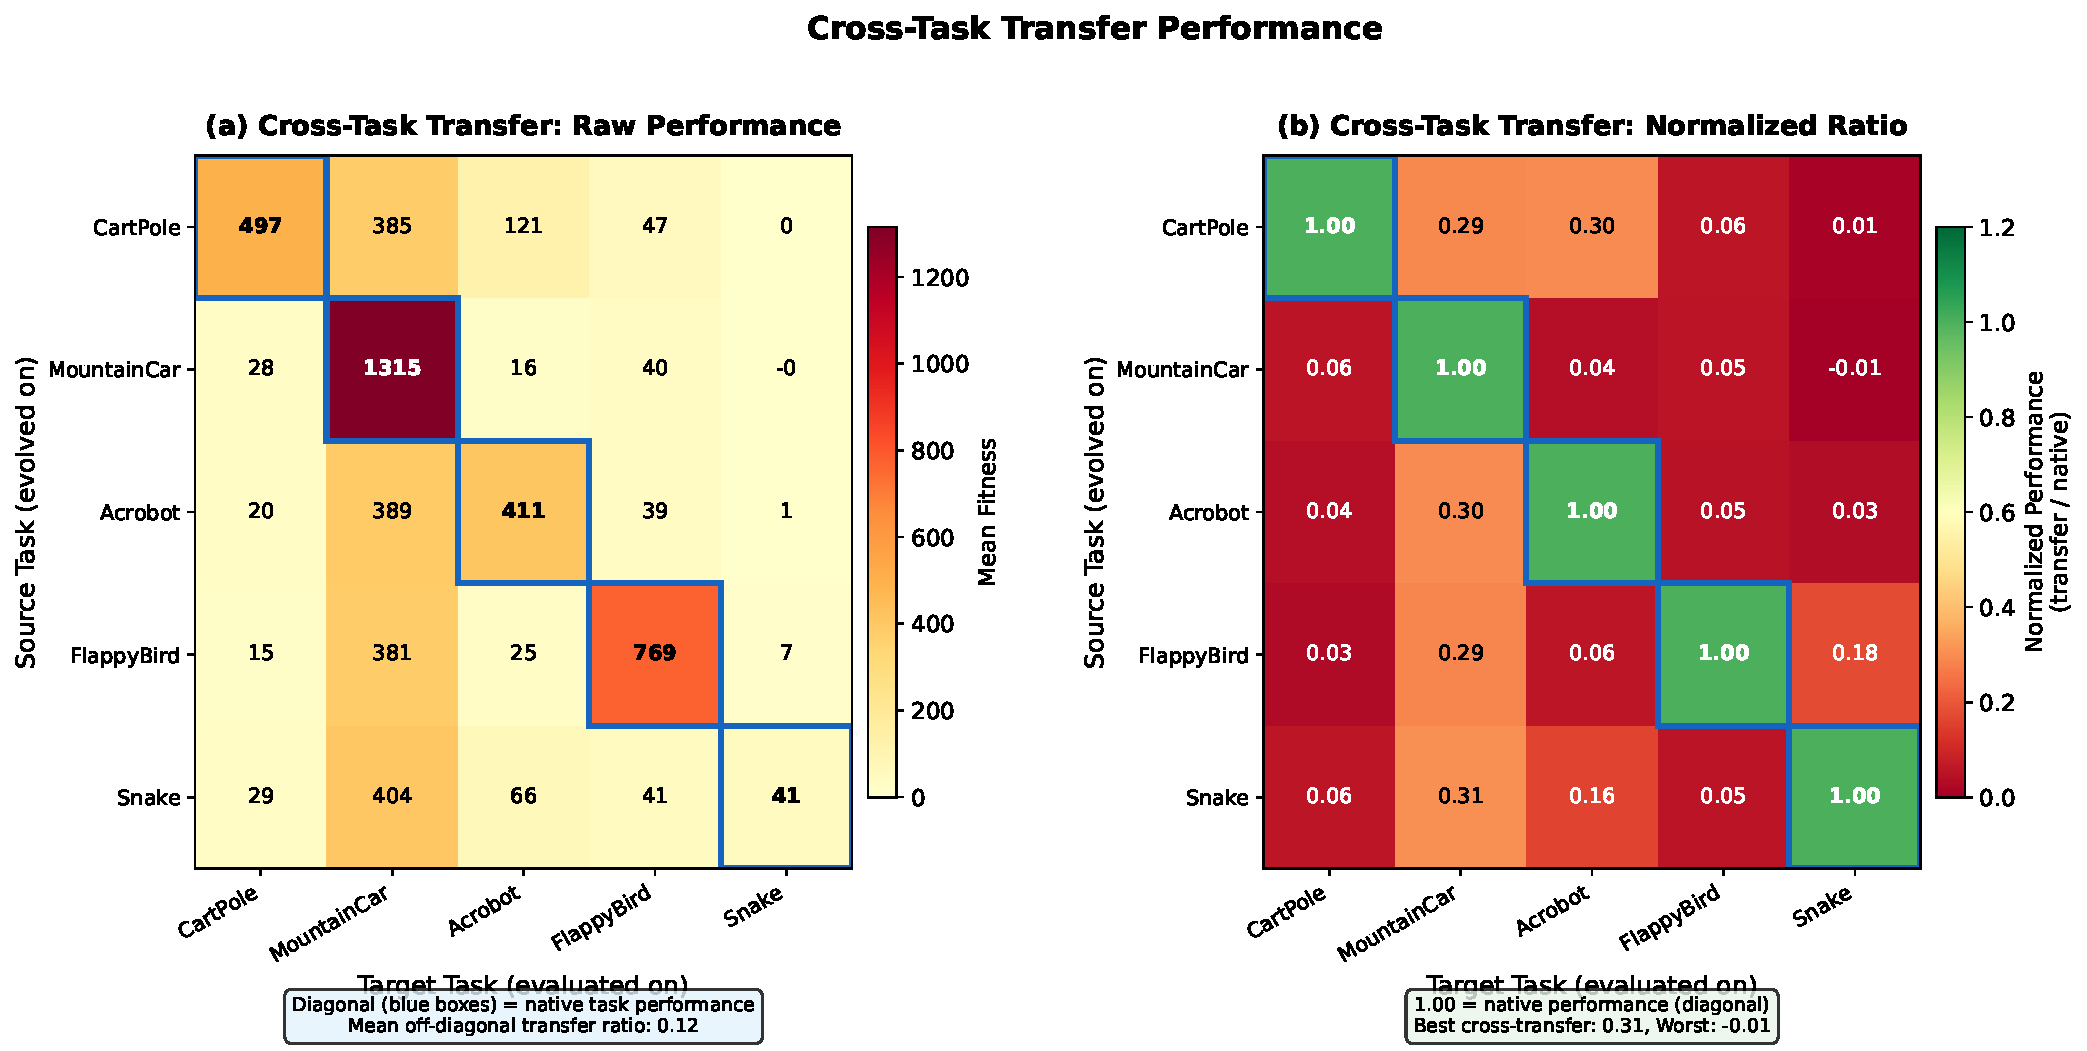
\includegraphics[width=0.92\linewidth]{figures_arxiv/fig10_cross_task.pdf}
\caption{\textbf{Cross-task transfer performance.} (a) Raw performance heatmap:
mean fitness when the topology evolved on the source task configuration (rows)
is embedded into and evaluated on the target task configuration (columns).
Diagonal entries show native task performance: CartPole~497,
MountainCar~1,315, Acrobot~411, FlappyBird~769, Snake~41. Mean off-diagonal
transfer is 0.12 and the best cross-transfer is 0.31. (b) Normalized ratio
heatmap: transfer fitness divided by native fitness.}
\end{figure}

\begin{figure}[H]
\centering
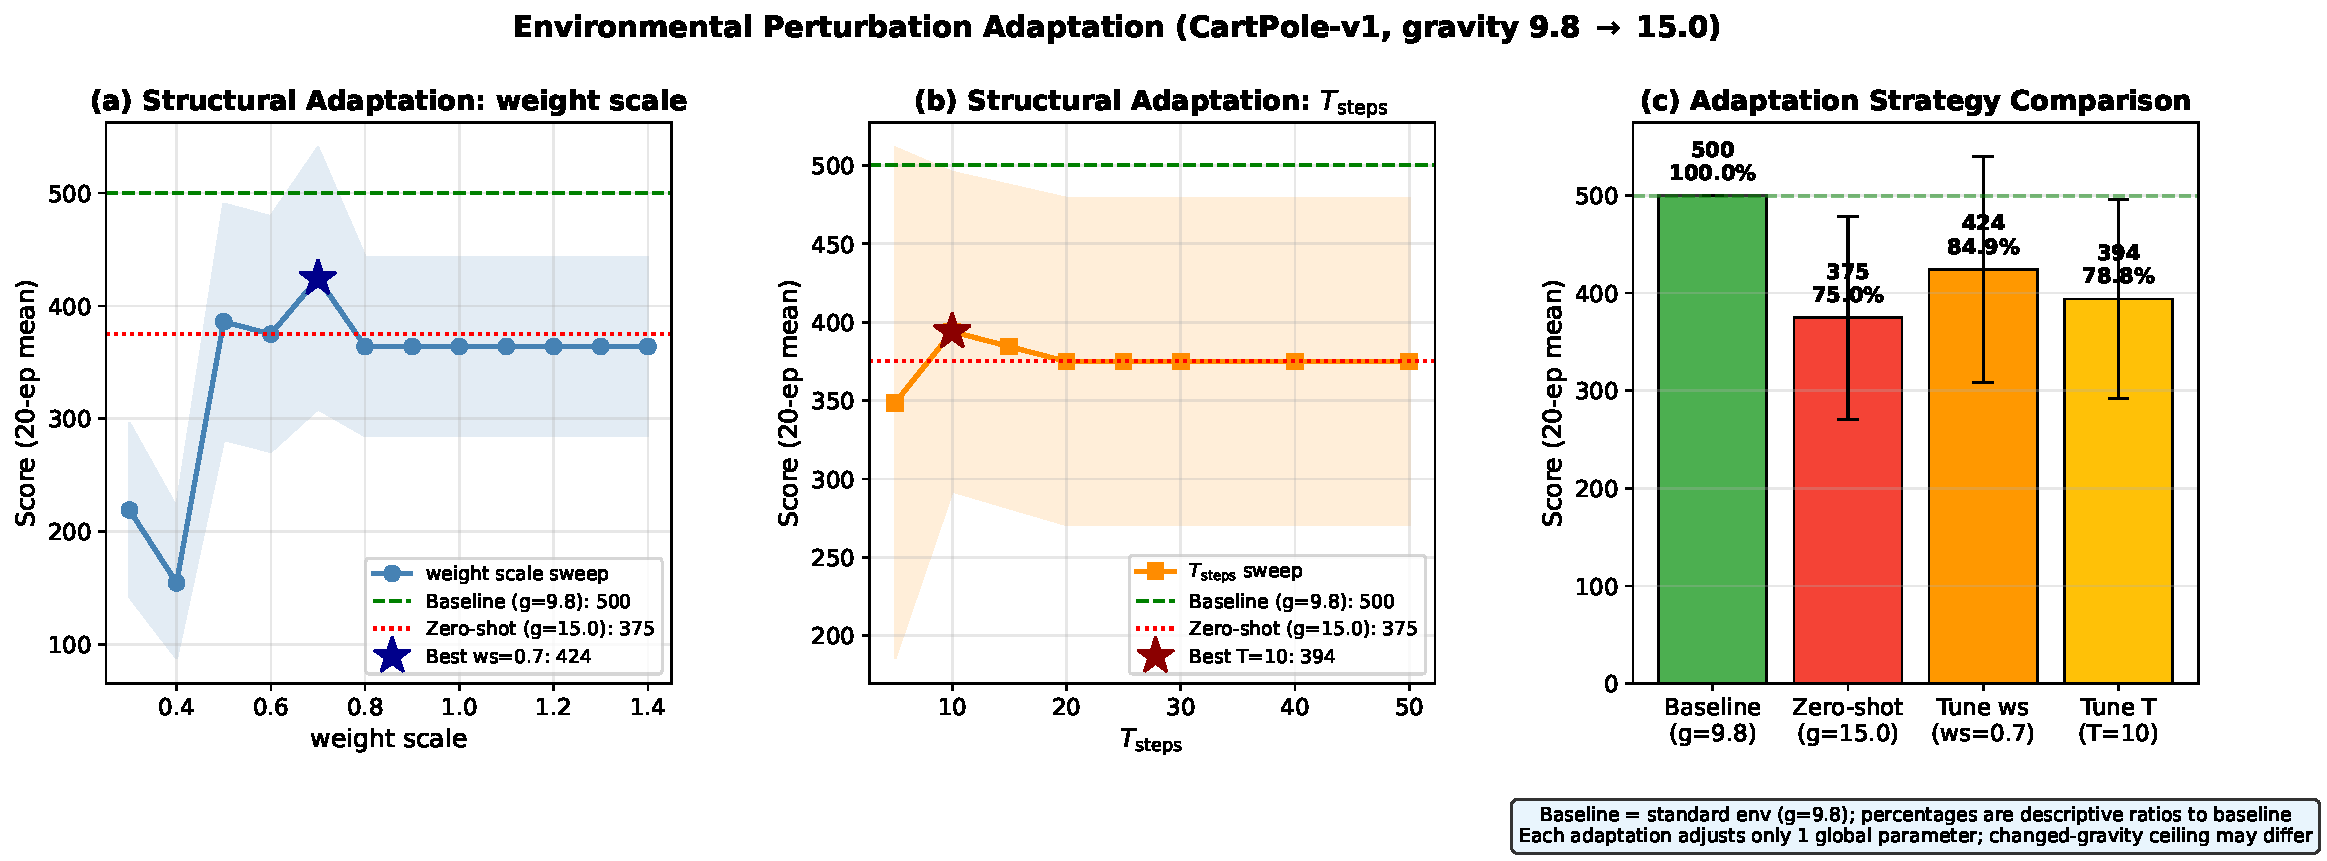
\includegraphics[width=0.92\linewidth]{figures_arxiv/fig09_adaptation.pdf}
\caption{\textbf{Comparison of adaptation strategies to abrupt environmental
change.} CartPole gravity is raised from 9.8 to 15.0. Baseline at standard
gravity is $500$; zero-shot performance at gravity 15.0 is $375$; global-scale
adaptation reaches $424$; $T_\text{steps}$ adaptation reaches $394$.}
\end{figure}

\section*{S6. HalfCheetah Boundary Audit}

\begin{table}[H]
\centering
\small
\caption{\textbf{HalfCheetah-v4 escape attempts.} The pre-specified boundary
threshold is $-200$. The best attempt improves the score to $-227.4$ but does not
cross the threshold, supporting the main-text statement that 6D action control is
a boundary of the present one-scale, 64--128 neuron setting rather than a proficiency-level benchmark.}
\begin{tabular}{@{}lc@{}}
\toprule
\textbf{Condition} & \textbf{Score} \\
\midrule
Random baseline & $-314.6$ \\
Original topology-only GA & $-415.5$ \\
Quality-diversity search & $-260.5$ \\
Fitness shaping & $-328.9$ \\
Larger population & $\mathbf{-227.4}$ \\
Per-output scales & $-241.3$ \\
Boundary threshold & $-200.0$ \\
\bottomrule
\end{tabular}
\end{table}

\end{document}


